\documentclass[12pt]{article}
\usepackage[english]{babel}
\usepackage{natbib}
\usepackage{url}
\usepackage[utf8x]{inputenc}
\usepackage{amsmath}
\usepackage{graphicx}
\graphicspath{{images/}}
\usepackage{parskip}
\usepackage{fancyhdr}
\usepackage{vmargin}
\usepackage{xcolor}
\usepackage{siunitx}
\usepackage{physics}
\setmarginsrb{3 cm}{2 cm}{3 cm}{2 cm}{1 cm}{1.5 cm}{1 cm}{1.5 cm}

\title{Lab 01}													% Title
\author{G 03}														% Author
\date{19 Mar 2019}														% Date

\makeatletter
\let\thetitle\@title
\let\theauthor\@author
\let\thedate\@date
\makeatother

\pagestyle{fancy}
\fancyhf{}
\rhead{\theauthor}
\lhead{\thetitle}
\cfoot{\thepage}
\newcommand{\mis}[3]{(#1 \pm #2) \ #3}
\newcommand{\misp}[3]{(#1 \#3 \pm #2}
\begin{document}

%%%%%%%%%%%%%%%%%%%%%%%%%%%%%%%%%%%%%%%%%%%%%%%%%%%%%%%%%%%%%%%%%%%%%%%%%%%%%%%%%%%%%%%%%

\begin{titlepage}
	\centering
    \vspace*{0.5 cm}
    
\includegraphics[scale = 0.75]{polito.jpg}\\[1.0 cm]				% University Logo
    \textsc{\LARGE Politecnico di Torino}\\[2.0 cm]						% University Name
	\textsc{\Large Digital systems electronics\\ A.A. 2018/2019}\\[0.5 cm]		% Course Code
	\textsc{\Large Prof. G. Masera}\\[0.5 cm]		% Nome del Professore
	\rule{\linewidth}{0.2 mm} \\[0.4 cm]
	{ \huge \bfseries \thetitle \\ \small \thedate}\\
	\rule{\linewidth}{0.2 mm} \\[1.5 cm]
	
	\begin{minipage}{0.4\textwidth}
		\begin{flushleft} \large
			Berchialla Luca\\												%Cognomi e nomi
			Laurasi Gjergji
			\\
			
			Mattei Andrea\\
            Lombardo Domenico Maria\\
            
			\end{flushleft}
			\end{minipage}~
			\begin{minipage}{0.4\textwidth}
            
			\begin{flushright} \large
			236032\\													%Matricole
			238259\\
            233755\\
            233959\\
            
		\end{flushright}
        
	\end{minipage}\\[2 cm]
	
\end{titlepage}

%%%%%%%%%%%%%%%%%%%%%%%%%%%%%%%%%%%%%%%%%%%%%%%%%%%%%%%%%%%%%%%%%%%%%%%%%%%%%%%%%%%%%%%%%

\section{ Controlling the LEDs }

The main purpose of the first point is to test the board and to get acquainted with the developing procedures for digital circuits on FPGAs using VHDL.\\
The task consisted in associate the 10 switches of DE1 board to its 10 LEDs.
The simple combinational circuit was tested using Modelsim with a simple testbench that simulated every switch one by one.\\
Quartus prime was used for compiling and loading the project on the board.
\section{2-to-1 Multiplexer}
As figure 1 shows we are implementing a 2-to-1 Multiplexer using a stuctural approach. Since its internal implementation its pretty trivial we will not discuss it any further.

\begin{figure}[h]
	\centering
	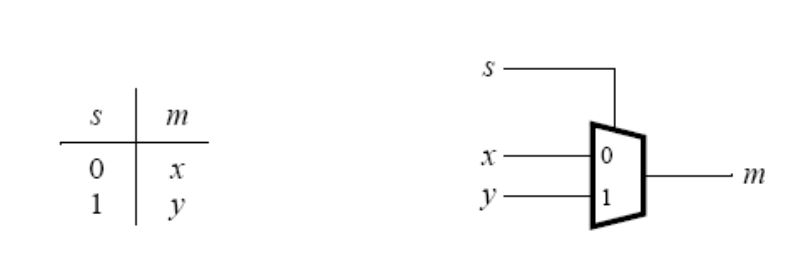
\includegraphics[scale = 0.5]{image2.jpg}
	\caption{multiplexer + truth table}
\end{figure}

Its VHDL code has been written under Quartus prime. Than a testbench was developed under modelsim. In the testbench we fixed the two multplexed inputs and than varing the selection bit we checked the behaviour.

After the simulation was succesful we impoted the pin assignements into Quartus prime and after compiling and loading it on the board we verified the actual behaviour.
\\\\
\section{5-to-1 Multiplexer}
\begin{figure}[h]
	\centering
	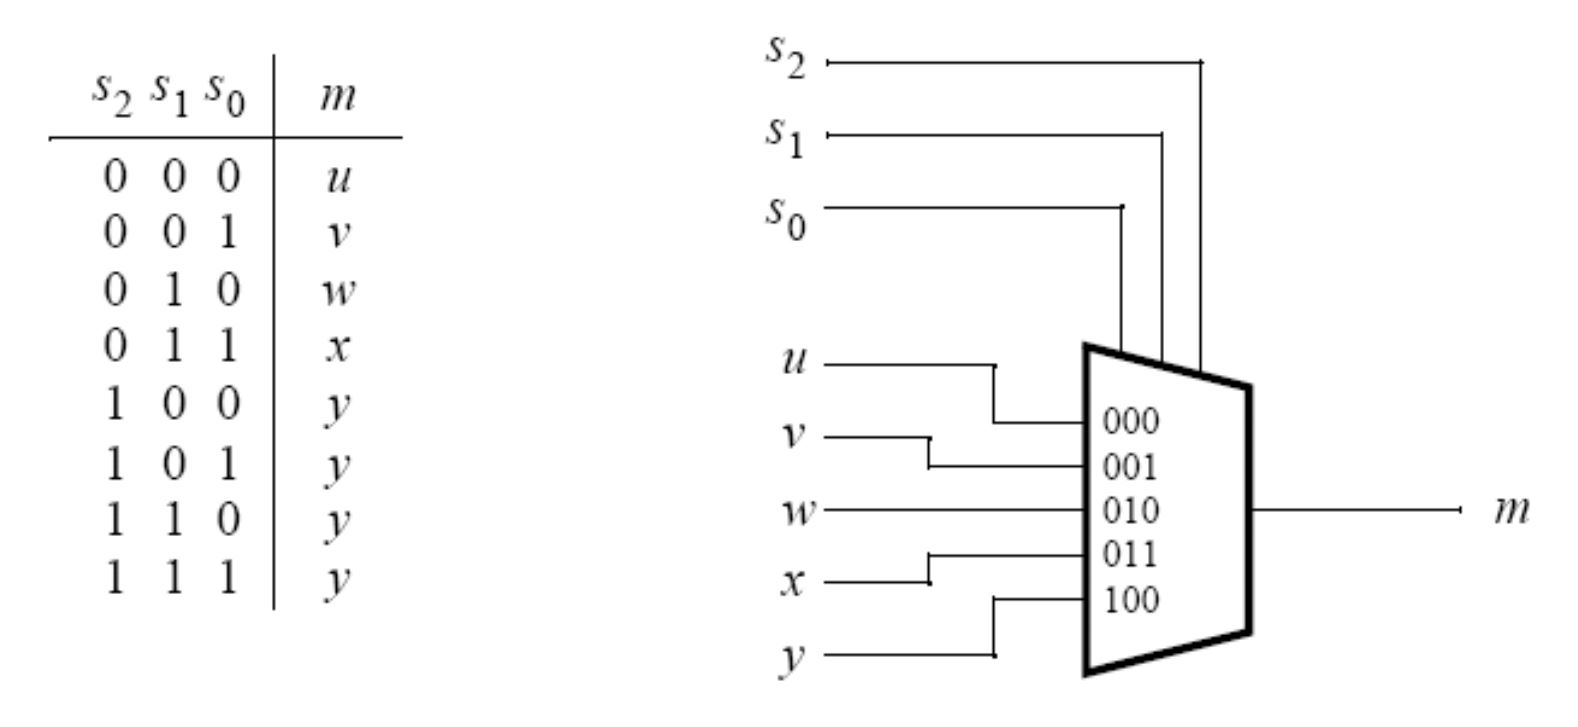
\includegraphics[scale = 0.3]{image1.jpg}
	\caption{multiplexer + truth table}
\end{figure}
We're now interested in designing the circuit shown in figure 2, where the output signal can be chosen between 5 different input signals with a 3 bit control signal as shown in the truth table. \\The circuit model has been implemented using a behavioural approach, that leads to a faster but less customizable solution to design a 5 to 1 MUX.\\
The circuit has been proved to work thanks to a testbech simulation, checking the correspondence of input-output following the already cited truth table. \\
Finally the vhdl code has been loaded into the hardware fpga showing positive results as expected by simulation.

\end{document}
